
% \begin{itemize}
%     \item \add{Descrição do ambiente experimental e das plataformas utilizadas (robôs, sensores, sistema OptiTrack e a plataforma LIMO, se aplicável).}
%     \item \add{Apresentação do SLAM\_toolbox: principais funcionalidades, justificativa para a escolha e forma de integração com o sistema de robôs.}
%     \item \add{Detalhamento da metodologia de comparação: critérios, métricas de desempenho (erro de localização, tempo de processamento, robustez, etc.) e a forma de coleta e análise dos dados.}
% \end{itemize}

% \add{Neste capítulo deverão ser descritos os recursos usados para a realização do projeto (equipamentos, material bibliográfico, programas de simulação, etc.), bem como aspectos relativos à disponibilidade ou não dos mesmos para a realização do estudo. Caso a disponibilidade de algum recurso seja limitada, ou esteja vinculada a alguma data de entrega, fator externo ou, até mesmo, a outro projeto, tal informação deve ser apresentada de forma explícita e clara nesta seção. O atraso ou a indisponibilidade deste recurso afetará diretamente o cronograma de execução do projeto, fato que deve ser cuidadosamente avaliado na construção do cronograma.}

\label{Cap03:Metodologia}
%% ----------------------------------------------
%%
%% -                  RECURSOS                  -
%%
%% ----------------------------------------------
Este projeto se propõe a utilizar a \textbf{SLAM Toolbox} para localização e mapeamento de robôs móveis terrestres no ambiente do Laboratório de Automação Inteligente e Robótica (LAB-AIR) e analisar a qualidade do posicionamento e do controle utilizado para os robôs desenvolverem trajetórias definidas, usando o sistema de câmeras OptiTrack presente no laboratório como referência de alta precisão (\textit{ground-truth}).

Para isso, utilizou-se da estrutura pré-existente do LAB-AIR, que dispõe de robôs móveis terrestres e aéreos, além de um sistema de câmeras OptiTrack empregado como referência de alta precisão (\textit{ground-truth}) na verificação do desempenho dos algoritmos de localização. 
Nas seções seguintes, serão apresentados os recursos e equipamentos utilizados, detalhando as características da plataforma robótica, dos sensores empregados e as especificidades do sistema de câmeras. A seção \ref{sec:ROS} discute aspectos relevantes do ecossistema ROS e da \textit{SLAM Toolbox}, que fundamentam a metodologia adotada neste projeto.


\section{Sistemas de Câmeras \textit{OptiTrack}}
\label{sec:Sistema_Optitrack}

    O LAB-AIR conta com um sistema de captura de movimento da \textit{OptiTrack} que é utilizado como um sistema de referência para a pose do robô, devido à sua alta resolução e precisão. Este sistema consiste em doze câmeras \textit{Full HD} de alta velocidade capazes de identificar a posição de marcadores reflexivos acoplados na parte externa do robô com precisão milimétrica e taxa de aquisição de até 240 frames por segundo (fps). As câmeras estão conectadas a um computador com \textit{Windows 10} rodando o software \textit{Motive} \cite{site:OptiTrack_Motive}, responsável por processar as informações individuais das câmeras e disponibilizar as informações de posicionamento dos marcadores detectados pelas câmeras. No software é possível selecionar todos os marcadores que estão acoplados ao robô, unificá-los como um objeto e nomeá-los para identificação, o que permite obter tanto a posição quanto a orientação de um ou mais objetos.
    
    \begin{figure}[htb]
         \centering
         \caption{Arena do LAB-AIR.}
         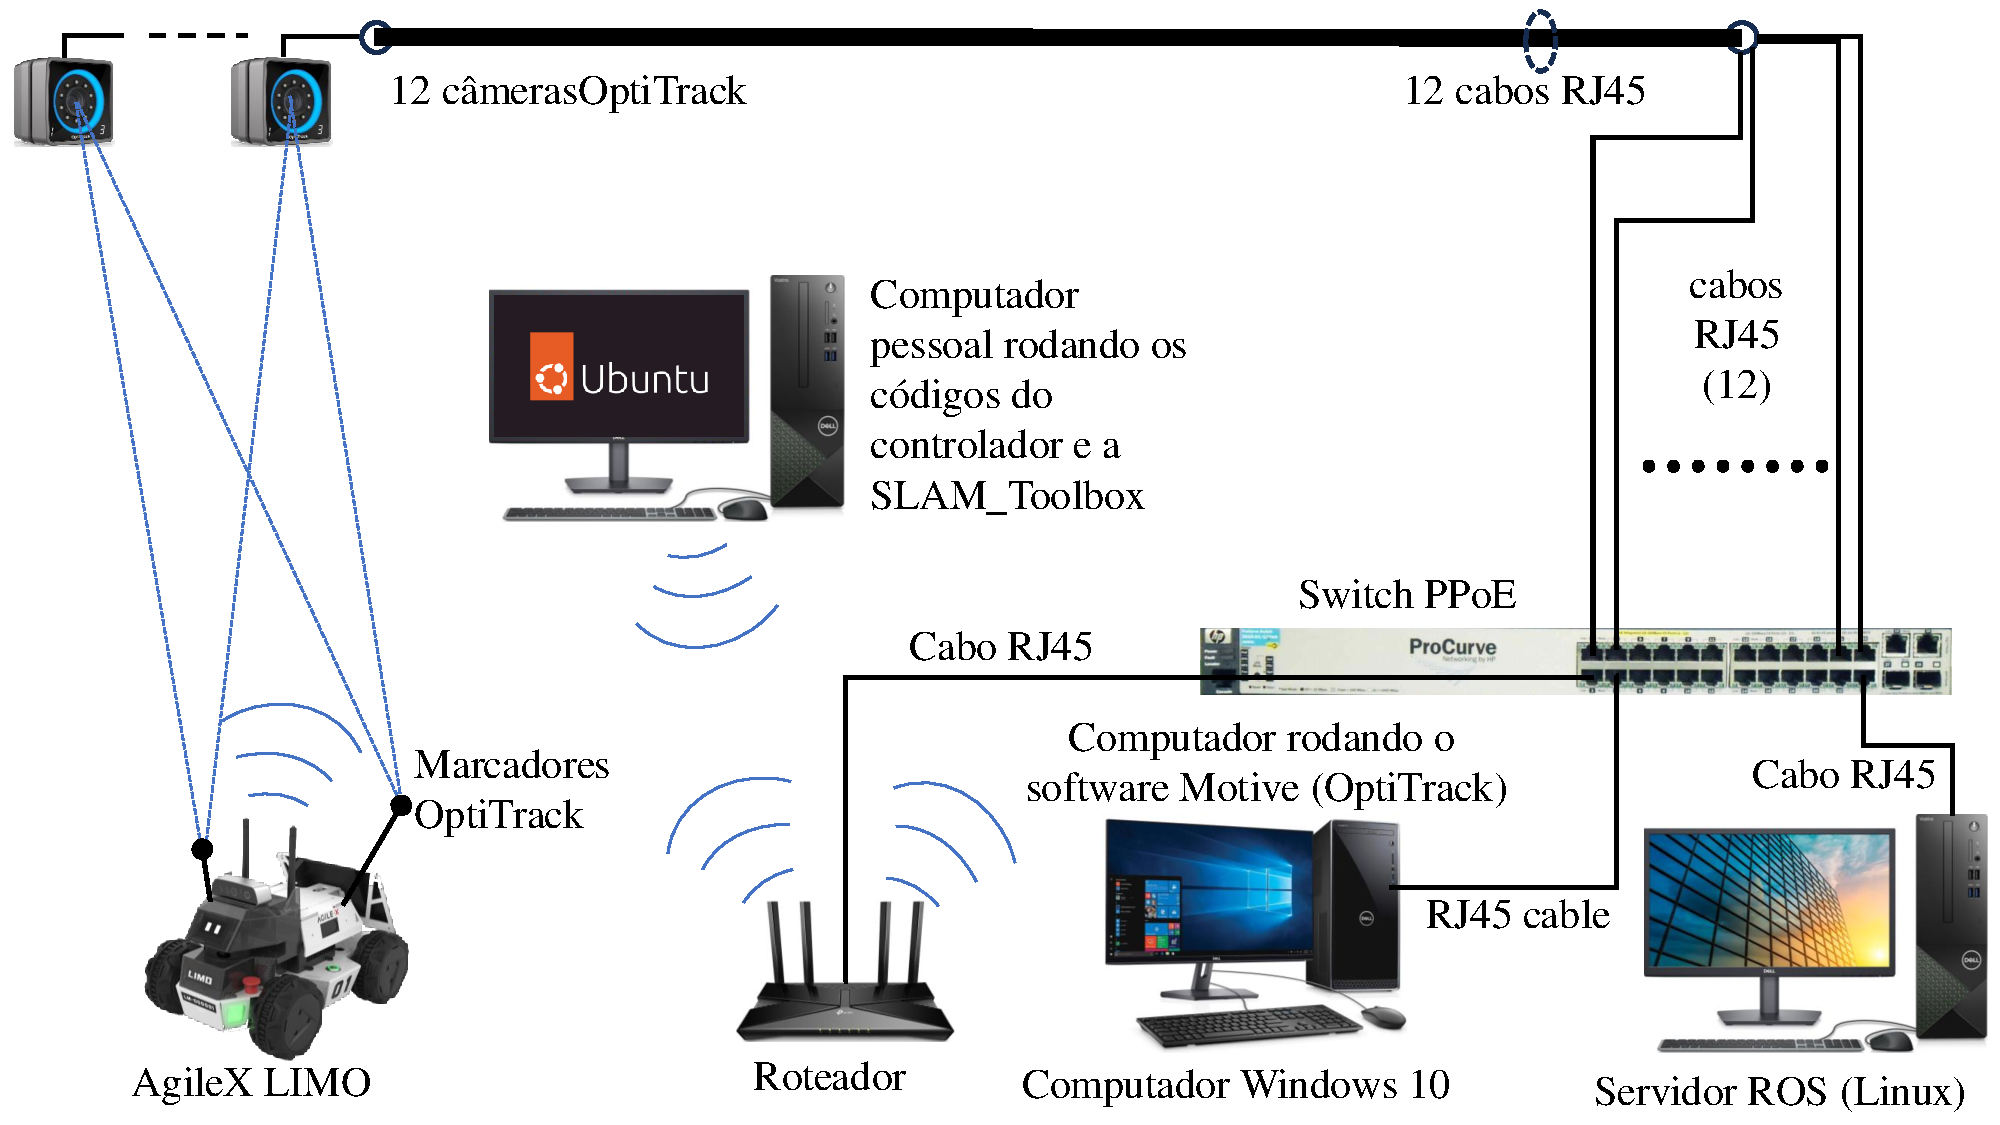
\includegraphics[width=\linewidth]{img/OptitrackArenaTCC_Mauricio.pdf}
         \source
         \label{fig:ArenaLAB-AIR}
     \end{figure}
    
    Este computador rodando o \textit{Motive} também se conecta, via uma rede local (não conectada à internet), com outro computador rodando Linux (Ubuntu 18.04) com o ROS Melodic instalado, o que permite que os dados capturados pelas câmeras e processados pelo \textit{Motive} sejam disponibilizados na rede do sistema ROS ao utilizar o pacote \textit{vrpn\_client\_ros}, que estabelece uma comunicação através do protocolo VRPN (\textit{Virtual-Reality Peripheral Network}). Estes pacotes permitem que a posição e a orientação dos objetos e corpos rígidos criados no \textit{Motive} e detectados sejam publicados em tópicos específicos e utilizados por outros pacotes ROS conectados à mesma rede.


\section{Plataforma Robótica LIMO}
\label{sec:Plataforma_LIMO}

    Como plataforma móvel principal foi utilizado o robô móvel terrestre \textit{LIMO}, desenvolvido pela \textit{Agilex Robotics}\cite{site:Agilex_Robotics}. Esta é uma plataforma versátil, contando com quatro diferentes modos de operação (diferencial, com esteiras, omnidirecional e \textit{Ackermann}) e equipada com sensores de percepção ativos, contando com um sensor laser do tipo \textit{LiDar} e uma câmera de profundidade, imprescindíveis para a execução de tarefas de mapeamento e localização do robô no seu entorno. A Figura \ref{fig:LIMO_MODES} apresenta o robô LIMO em configurações diferentes de montagens para uso nos diversos modos de operação disponíveis. A imagem mais à direita mostra a montagem usada no modo diferencial e \textit{car-like}.

    \begin{figure}[htb]
        \centering
        \caption{Plataforma Robótica LIMO em seus diferentes modos de operação. À esquerda, configuração omnidirecional com rodas \textit{mecanum}. Ao centro, configuração com esteiras e à direita, robô com as rodas padrão para uso nas configurações \textit{Ackermann} ou diferencial.}
        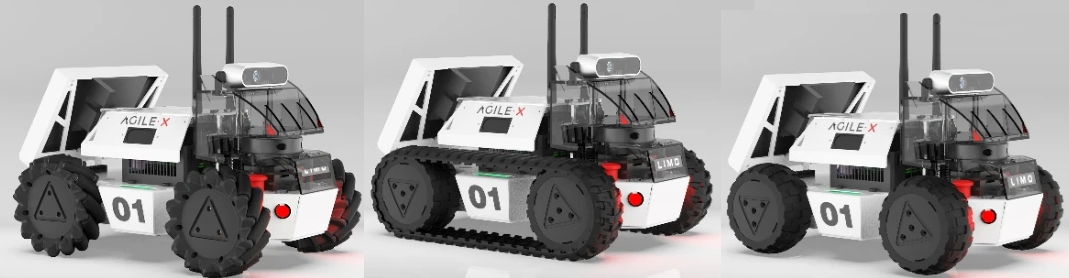
\includegraphics[width=\linewidth]{img/Limo_modes.png}
        \label{fig:LIMO_MODES}
        \source[\cite{limoUserManual}]
    \end{figure}

    \subsection{Recursos Computacionais}
    \label{sec:Recursos_LIMO}
        O robô LIMO possui boa capacidade computacional a bordo e sensores adequados para estudos relacionados a navegação autônoma, SLAM, mapeamento, planejamento de trajetórias, desvio de obstáculos, etc. Sua bateria de 12V e 5200mAh fornece autonomia de 40 min de funcionamento ativo e até 2 horas em \textit{stand-by}. A Tabela \ref{tab:sensors_limo} mostra uma lista de alguns sensores/características desse robô.

        \begin{table}[htb]
        \centering        
        \caption{Lista de Sensores e características do LIMO}
            \resizebox{0.9\columnwidth}{!}{ % Resize to the column width
                \setlength{\extrarowheight}{4pt}            
                \begin{tabular}{|l|r|}
                     \hline
                     \textbf{Item} & \textbf{Descrição}\\ 
                     \hline
                     Dimensão Geral & $322\ mm\times220\ mm\times251\ mm$\\ \hline
                     Placa Principal & NVIDIA Jetson Nano (4G)\\ \hline
                     Sistema Operacional & Ubuntu 18.04\\ \hline
                     Sensor Laser & YDLiDAR EAI X2L\\ \hline
                     Camera de Profundidade & ORBBEC Astra+\\ \hline
                     Unidade de Medição Inercial & HI226\\ \hline
                     Módulo de Voz & iFlytek assistente de voz\\ \hline
                     Auto-falantes & Esquerdo e Direito, \textit{Dual Channel} (2x2W)\\ \hline
                     Hub USB & Um USB tipo C e duas portas USB 2.0 \\ \hline
                     \textit{Display} Frontal & 1.54 pol. 128x64 \textit{display} OLED branco \\ \hline
                     \textit{Display} Traseiro & 7 pol. 1024x600 IPS \textit{touch screen}\\ \hline
                     Comunicação & Wi-Fi e Bluetooth 5.0 \\ \hline
                     Velocidade Máxima sem carga & $\pm\ 1\ m/s,$ sem carga\\ \hline
                     Bateria & 12 V Li-ion, 5200 mAh\\ \hline
                     Duração da bateria em uso & 40 minutes \\ \hline
                     Duração da bateria em \textit{stand-by} & 2 hours \\ 
                     \hline
                \end{tabular}
            }
        \source[Adaptado de \cite{limoUserManual}]
        \label{tab:sensors_limo}
    \end{table}

        A placa principal, uma Nvidia Jetson Nano, é um computador de pequeno porte poderoso capaz de suportar aplicações diversas assim como aplicações de IA de nível básico. Ela possui uma CPU Quad-Core ARM57 de 64 bits rodando a 1,43 GHz, 4 GB de memória RAM LPDDR4 e uma GPU Nvidia Maxwell de 128 núcleos, capaz de decodificação de vídeo em resolução 4K a 60 quadros por segundo. A placa possui um conector Ethernet Gigabit para acesso rápido à internet, saída HDMI, 4 portas USB 3.0, que permitem a conexão de vários dispositivos, e uma porta USB 2.0 Micro-B para alimentação.

        O chassi do LIMO é feito de chapas metálicas, pesa cerca de 4,8 kg e suporta até 4 kg de carga útil. Além disso, essa estrutura pode ser expandida para integrar uma unidade de processamento mais poderosa ou outros dispositivos de sensoriamento. Ou seja, o hardware nativo do LIMO é expansível, o que o torna ainda mais interessante para pesquisa/aplicações. O robô também conta com um módulo Bluetooth 5.0 embutido para conexão com um aplicativo móvel disponível para Android. O LIMO e a placa Jetson Nano estão diretamente conectados por meio de uma interface UART, e a placa pode controlar o chassi através dessa interface. O hub USB fornece duas interfaces tipo A e uma interface Tipo C, todas operando sob o protocolo USB 2.0. A tela traseira é conectada ao hub USB através da interface USB 2.0 e possui função de toque.

        A placa Nvidia Jetson Nano executa o Ubuntu 18.04, e utiliza o SDK Nvidia JetPack, que contém bibliotecas para aprendizado profundo, visão computacional, gráficos e multimídia. O driver do LIMO, responsável pela comunicação computador de bordo-chassis, foi desenvolvido usando o sistema ROS (Robot Operating System), o que facilita a interação com outros sistemas ROS ao realizar tarefas de forma autônoma. Ele possui duas versões, em C++ e em Python, ambas podendo controlar o movimento do robô. A versão em Python está disponível no Python Package Index (PyPI)~\cite{limoRosPy}, e pode ser baixada usando o comando \texttt{pip}. A versão em C++ está disponível no Github \cite{limoRos1}.


    \subsection{Sensores}
    \label{sec:Sensores_LIMO}
        Como mostra a Tabela~\ref{tab:sensors_limo}, o LIMO possui um sensor LiDAR e uma câmera RGBD. O LiDAR, um YDLIDAR X2, é um sensor laser 2D de 360$^\circ$ que opera com frequência de varredura de 3 kHz e frequência de escaneamento de 6 Hz, com um alcance de até 8 metros em ambientes internos. 
        A câmera de profundidade ORBBEC ASTRA+ utiliza tecnologia de imagem 3D por luz estruturada binocular. Ela contém uma câmera RGB e uma câmera infravermelha, e pode medir profundidades de 0,3 a 3 metros, com uma precisão de 6 mm na faixa de 1 m e um atraso de 30 a 45 ms. Sua resolução máxima de mapa de profundidade é de 640x400 pixels e sua resolução máxima de mapa de cores é de 1920x1080 pixels, ambos a 30 quadros por segundo.
    
        A Unidade de Medição Inercial (IMU) HI226 de 6 graus de liberdade (6DoF) embarcada no LIMO combina um acelerômetro triaxial, um giroscópio triaxial e um microprocessador, permitindo adquirir dados de movimento em três eixos (X, Y e Z) com alta precisão (±2000°/s para o giroscópio e até ±8g para o acelerômetro), fornecendo excelente desempenho em diversas condições operacionais. Ela funciona à frequência máxima de saída, 100Hz, e utiliza algoritmos avançados de fusão de dados, podendo fornecer, simultaneamente, velocidades angulares e acelerações nos três eixos, quatérnios e ângulos de Euler, com pouca distorção de fase. Os erros (RMS) de inclinação e guinada são de 0,8° estáticos e 2,5° dinâmicos.


    \subsection{Controle do LIMO no modo Diferencial}
    \label{sec:Controle_Dif_LIMO}
    
        O controlador cinemático utilizado para o modo diferencial do LIMO é apresentado a seguir, baseado no controlador apresentado na seção \ref{sec:Modelo_Robos_Diferenciais}.
        
        Como o LIMO possui controladores de baixo nível incorporados ao robô, estes já convertem os comandos de velocidade recebidos em comandos de rotação das rodas. Portanto, precisamos apenas desenvolver um controlador de alto nível que calcule a velocidade longitudinal e a velocidade angular que desejamos que o robô desenvolva para atingir o objetivo. Consequentemente, o sinal de controle de alto nível utilizado é um vetor de velocidades $\begin{bmatrix}v & \omega \end{bmatrix}^{T}$.
        
        Os sensores do sistema provêm a última posição $\bs{x_c}$ do robô, então utiliza-se uma lei de controle \textit{feedforward} e \textit{feedback} proporcional, calculando-se o erro de posição do robô e a velocidade desejada do robô no objetivo, a saber,
        \begin{equation}
            \dot{\bs{x}}_{c,ref} = \dot{\bs{x}}_{c,des} + \bs{\kappa}(\bs{x}_{c,des} - \bs{x}_c),
            \label{eq:ff_fb_law_limo}
        \end{equation}
        em que $\bs{\kappa}$ é uma matriz diagonal definida positiva, $\dot{\bs{x}}_{c,des}$ é o vetor de velocidades desejadas e $\dot{\bs{x}}_{c,ref}$ é o vetor de velocidades que o robô deve executar no referencial inercial do mapa ou do mundo.
    
        Como visto na seção \ref{sec:Modelo_Robos_Diferenciais}, o modelo cinemático do robô diferencial, \( \dot{\bs{x}}_c = \bs{H} \bs{u} \), é dado pela equação
        
        \begin{equation}
            \begin{bmatrix} \dot{x}_c \\ \dot{y}_c  \end{bmatrix} = \begin{bmatrix} \cos{\psi} & -a \sin{\psi} \\ \sin{\psi} & a \cos{\psi}   \end{bmatrix} \begin{bmatrix} v \\ \omega    \end{bmatrix}
            \label{eq:kinematics_differential_limo}
        \end{equation}
        
        e podemos obter o controlador cinemático diretamente pela cinemática inversa \cite{Sarcinelli-Filho2023_4}, tal que $\bs{u} = \bs{H}^{-1} \dot{\bs{x}}_{c,ref}$, ou seja,
        
        \begin{equation}
           \begin{bmatrix} v \\ \omega    \end{bmatrix}
           =  
           \begin{bmatrix} \cos{\psi} & \sin{\psi} \\ -\frac{1}{a}\sin{\psi} & \frac{1}{a} \cos{\psi}   \end{bmatrix} 
           \begin{bmatrix}\dot{x}_{c,ref} \\ \dot{y}_{c,ref}   \end{bmatrix}
           \label{eq:kinematic_controller_differential_limo}
        \end{equation}
        
        onde $v$ e $\omega$ são, respectivamente, as velocidades linear e angular no sistema de coordenadas do robô e, consequentemente, os sinais de controle que são enviados para controlá-lo.
    


\section{ROS - Robot Operating System}
\label{sec:ROS}

    

    \subsection{Pacotes ROS e Launchers do LIMO}
    \label{sec:ROS_LIMO}
            
        A Agilex fornece pacotes do LIMO contendo o \textit{driver} C++, arquivos de configuração, \textit{launchers} ROS e modelos URDF em seu repositório oficial no GitHub~\cite{GithubAgilex} para ambas as versões do ROS \cite{limoRos1,limoRos2}. O pacote \texttt{limo\_base} contém o \textit{driver} em C++, que oferece a interface principal necessária para comunicar com o robô, obter informações de odometria e enviar comandos de velocidade. O \textit{launcher} ROS para inicializar o driver é o \texttt{limo\_base.launcher}.
        
        O pacote \texttt{limo\_bringup} oferece diversos \textit{launchers} para inicializar os recursos disponíveis no robô. O \textit{launcher} \texttt{limo\_start.launch} inicializa o \texttt{limo\_base} e o LiDAR, além de definir a árvore de transformadas entre a base do robô, a câmera, a IMU e o laser. Este pacote também contém outros \textit{launchers} para execução de algoritmos de mapeamento, navegação, visualização, entre outros.
    
        Como observação, no pacote ROS \texttt{limo\_base} fornecido pelo fabricante, o comando de velocidade linear $v$ e o comando de velocidade angular $\omega$ são publicados sob o tópico \texttt{cmd\_vel}, e essas velocidades devem ser atribuídas em \texttt{linear.X} e \texttt{angular.Z}, respectivamente.

    \subsection{Biblioteca Slam Toolbox}
    \label{sec:SLAM_Toolbox}

    % \add{Apresentação do SLAM\_toolbox: principais funcionalidades, justificativa para a escolha e forma de integração com o sistema de robôs.}
    
    % \add{Detalhamento da integração do SLAM\_toolbox com os demais módulos do sistema (por exemplo, aquisição e fusão dos dados sensoriais, controle do robô).}

    De acordo com \citeonline{Macenski2021}, a SLAM Toolbox nasceu com o foco em lidar com ambientes dinâmicos e de grande escala, como galpões, indústrias ou hipermercados, utilizando os processadores limitados presentes em robôs móveis. Segundo eles, os algoritmos de SLAM \textit{open-source} existentes anteriormente no ambiente ROS não eram capazes de realizar o mapeamento correto de grandes áreas e o único que era capaz de fazê-lo, o \textit{Cartographer}, foi abandonado pelo Google e não recebe mais atualizações e melhorias.

    A SLAM Toolbox foi construída sobre a base do algoritmo Open Karto (da SRI \textit{International}), incorporando técnicas modernas de otimização. Utiliza um método de SLAM baseado em grafos (\textit{graph-based}), em que o mapa é representado por um grafo de poses do robô conectadas por restrições de odometria e detecções de loop (fechamento de ciclo), diferindo dos métodos baseados em filtros de Bayes \cite{2023bayesian} (ex.: filtro de partículas do GMapping \cite{Grisetti2007}) \cite{Thrun2005}. Este método permite maior eficiência de recursos computacionais, especialmente enquanto realiza a construção de mapas em larga escala.

% ------------
    \subsubsection{Princípio de Funcionamento e Algoritmo}

    Em operação, a SLAM Toolbox executa um nó ROS que se subscreve aos dados de um sensor LiDAR 2D (mensagens do tipo \textbf{LaserScan}) e às transformações de odometria do robô(\textit{frame} odom $\rightarrow$ base\_link), produzindo como saída um mapa ocupacional 2D (\textit{frame} map) e a transformação estimada de localização do robô (map $\rightarrow$ odom). A cada varredura recebida do laser, o algoritmo calcula a pose relativa do robô (integrando a odometria) e associa a ela a leitura correspondente do laser, formando um objeto (\textit{PosedScan}) que é inserido em uma fila de processamento. Conforme o robô se move, novos nós são adicionados a um grafo de poses sempre que o deslocamento ultrapassa certos limiares mínimos de distância e/ou ângulo (parâmetros configuráveis) para garantir mudança significativa. Cada novo nó conecta-se ao anterior por uma aresta de odometria e, adicionalmente, é refinado por casamento de scans (scan matching) com a pose anterior, o que alinha a leitura laser atual com a esperada a partir do mapa em construção. O uso do algoritmo robusto de casamento de laser herdado do Open Karto garante alinhamento preciso das leituras sequenciais.

    Conforme o grafo se constrói, a SLAM Toolbox busca detecções de fechamento de loop (loop closures). Isso ocorre quando uma leitura atual do laser tem alta correlação com partes do mapa já mapeadas anteriormente, indicando que o robô retornou a uma região conhecida. Nesses casos, o algoritmo adiciona arestas no grafo conectando a pose atual com aquela pose passada correspondente (restrição de loop) e então executa uma otimização global do grafo para minimizar os erros acumulados. A otimização é realizada por métodos de mínimos quadrados não lineares; originalmente o Karto usava um otimizador de Sparse Bundle Adjustment, mas na SLAM Toolbox este foi substituído pelo solver Google Ceres, resultando em otimização mais rápida e flexível\cite{Macenski2021}. O sistema foi projetado de forma modular, permitindo inclusive carregar diferentes plugins de solver – por meio de uma interface dinâmica em tempo de execução – possibilitando substituição futura do algoritmo de otimização sem modificar o núcleo do código.

    Uma vez otimizado o grafo (especialmente após um fechamento de loop), todas as poses do robô são ajustadas consistentemente, e o mapa ocupacional é atualizado utilizando as leituras laser armazenadas em cada pose corrigida. Esse processo garante um mapa globalmente consistente, corrigindo distorções à medida que loops são fechados. Em resumo, a SLAM Toolbox segue o paradigma típico de SLAM gráfico: construção incremental do mapa com ajustes retroativos ocasionais via otimização de grafo, ao invés de manter múltiplas hipóteses simultâneas como nos métodos de filtro de partículas.

    Um diferencial importante da SLAM Toolbox é suportar dois modos de operação quanto ao gerenciamento do fluxo de dados: síncrono e assíncrono. No modo síncrono, o nó processa todos os dados de sensor válidos na ordem em que chegam, podendo incorrer em atraso caso a taxa de leitura seja alta ou o processamento intenso (prioriza mapear com o máximo de detalhes). Já no modo assíncrono, o algoritmo processa os dados “o mais rápido possível”, descartando ou pulando leituras, se necessário, para manter o desempenho em tempo real (prioriza a responsividade). Esses modos permitem ajustar o funcionamento conforme a aplicação: por exemplo, em robôs com poder de computação limitado operando em áreas enormes, o modo assíncrono evita que o SLAM fique para trás em relação ao movimento do robô, enquanto em aplicações de mapping offline pode-se rodar no modo síncrono para utilizar todos os dados disponíveis. Em ambos os casos, o resultado final esperado (um mapa consistente) é equivalente, mas o modo assíncrono traz leve degradação de detalhe temporal para ganhar em robustez de tempo real. Adicionalmente, a biblioteca implementa um modo de operação apenas de odometria a laser (\textit{LiDAR odometry}), no qual é executada a mesma estimação de movimento por casamento de scans mas sem construir um mapa global – ou seja, sem um mapa prévio, o sistema atua como um odômetro local que realiza pequenos fechamentos de loop locais (útil para estimar movimento em tempo real quando não se deseja ainda um mapa completo). Esse modo pode ser entendido como uma forma degenerada de SLAM restrita a um mapa local temporário.

% --------
    
    A biblioteca conta com diversos modos de operação para SLAM e um modo de Localização que também pode ser utilizado para obter odometria através do sensor LiDAR quando nenhum mapa é carregado ao rodar o modo de Localização. 
    
    Utilizaremos o modo de operação online e síncrono da biblioteca para gerar o mapa do laboratório. Este modo de operação analisa todas as medições recebidas do sensor LiDAR, em ordem de recebimento, e faz a correlação entre a última medição recebida e medições anteriores em busca de correlações que permitam a localização do robô no mapa em construção e o fechamento de loops, que ocorrem quando a última medição corresponde bem o suficiente com medições passadas. O fechamento de loop é essencial para o mapeamento correto de ambientes, permitindo que o robô identifique que já esteve naquele local anteriormente.

    
    

    % \add{Descrição da implementação experimental, destacando as etapas de configuração, calibração e execução dos testes.}

    
\section{Detalhes da Implementação do Projeto}

    Para este projeto foi necessário realizar uma pequena modificação na estrutura do LIMO, modificando o local do seu sensor laser, que normalmente encontra-se montado na parte anterior do robô, possibilitando apenas o uso de $180\degree$ do campo de visão do LiDAR. Criou-se então uma plataforma para montagem do sensor laser na parte superior do corpo do robô, a fim de possibilitar o uso completo dos $360\degree$ do campo de visão do LiDAR do robô (Ver Figura \ref{fig:LIMO_Experimento}). 
    
    \begin{figure}[htb]
        \centering
        \caption{Modificação realizada no robô móvel para uso do campo de visão total do LiDAR. À esquerda, imagem do LIMO com o sensor na posição original. À direita, imagem do robô com a estrutura modificada.}

        \begin{subfigure}[b]{0.45\textwidth}
        \centering
            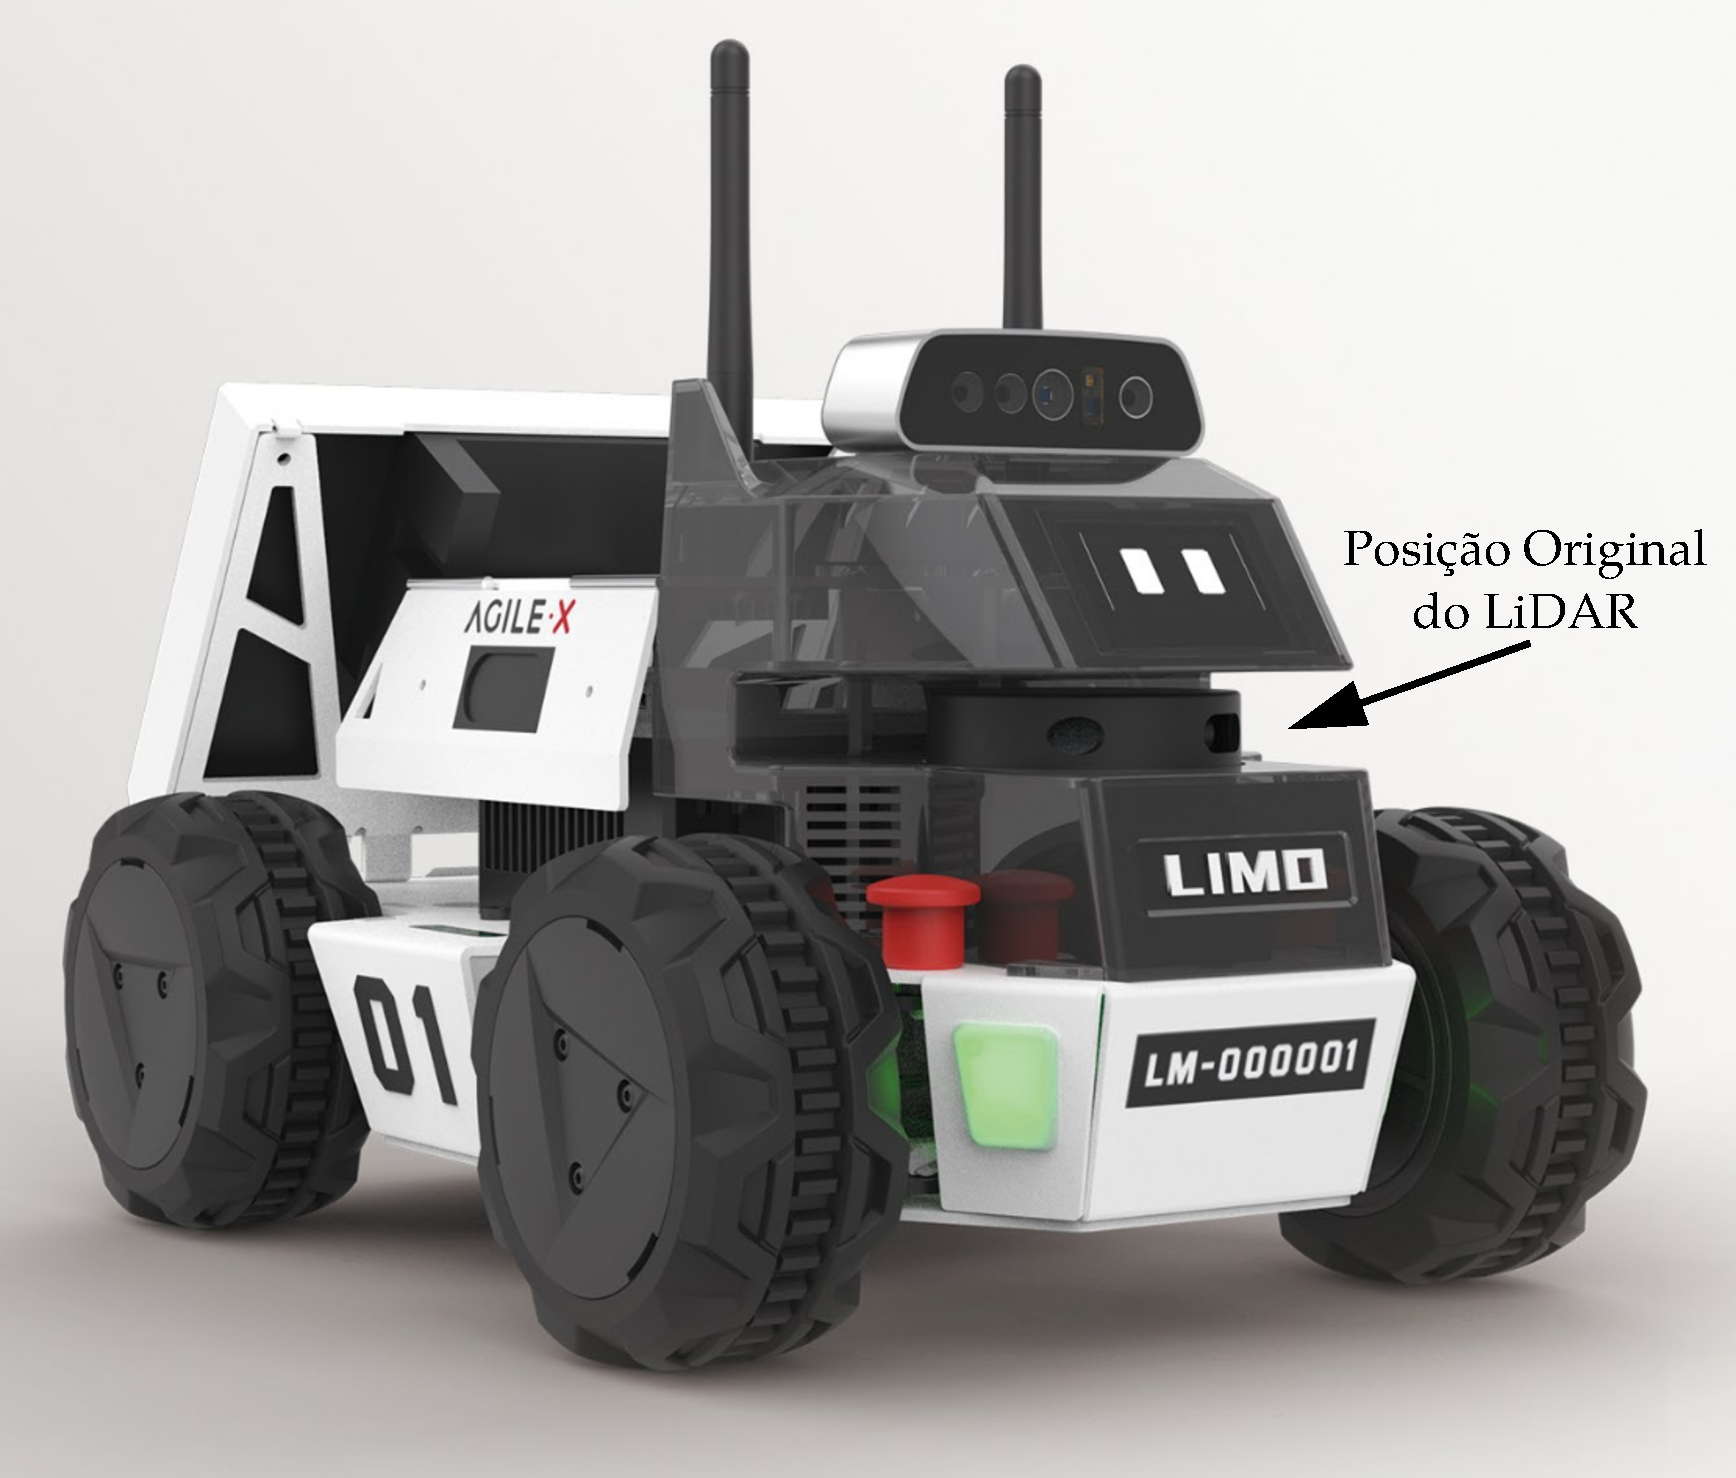
\includegraphics[height=0.94\textwidth, width=\textwidth]{img/LIMO_LiDAR_2.pdf}
            
        \end{subfigure}
        \hspace{0.03\textwidth}
        \begin{subfigure}[b]{0.45\textwidth}
        \centering
            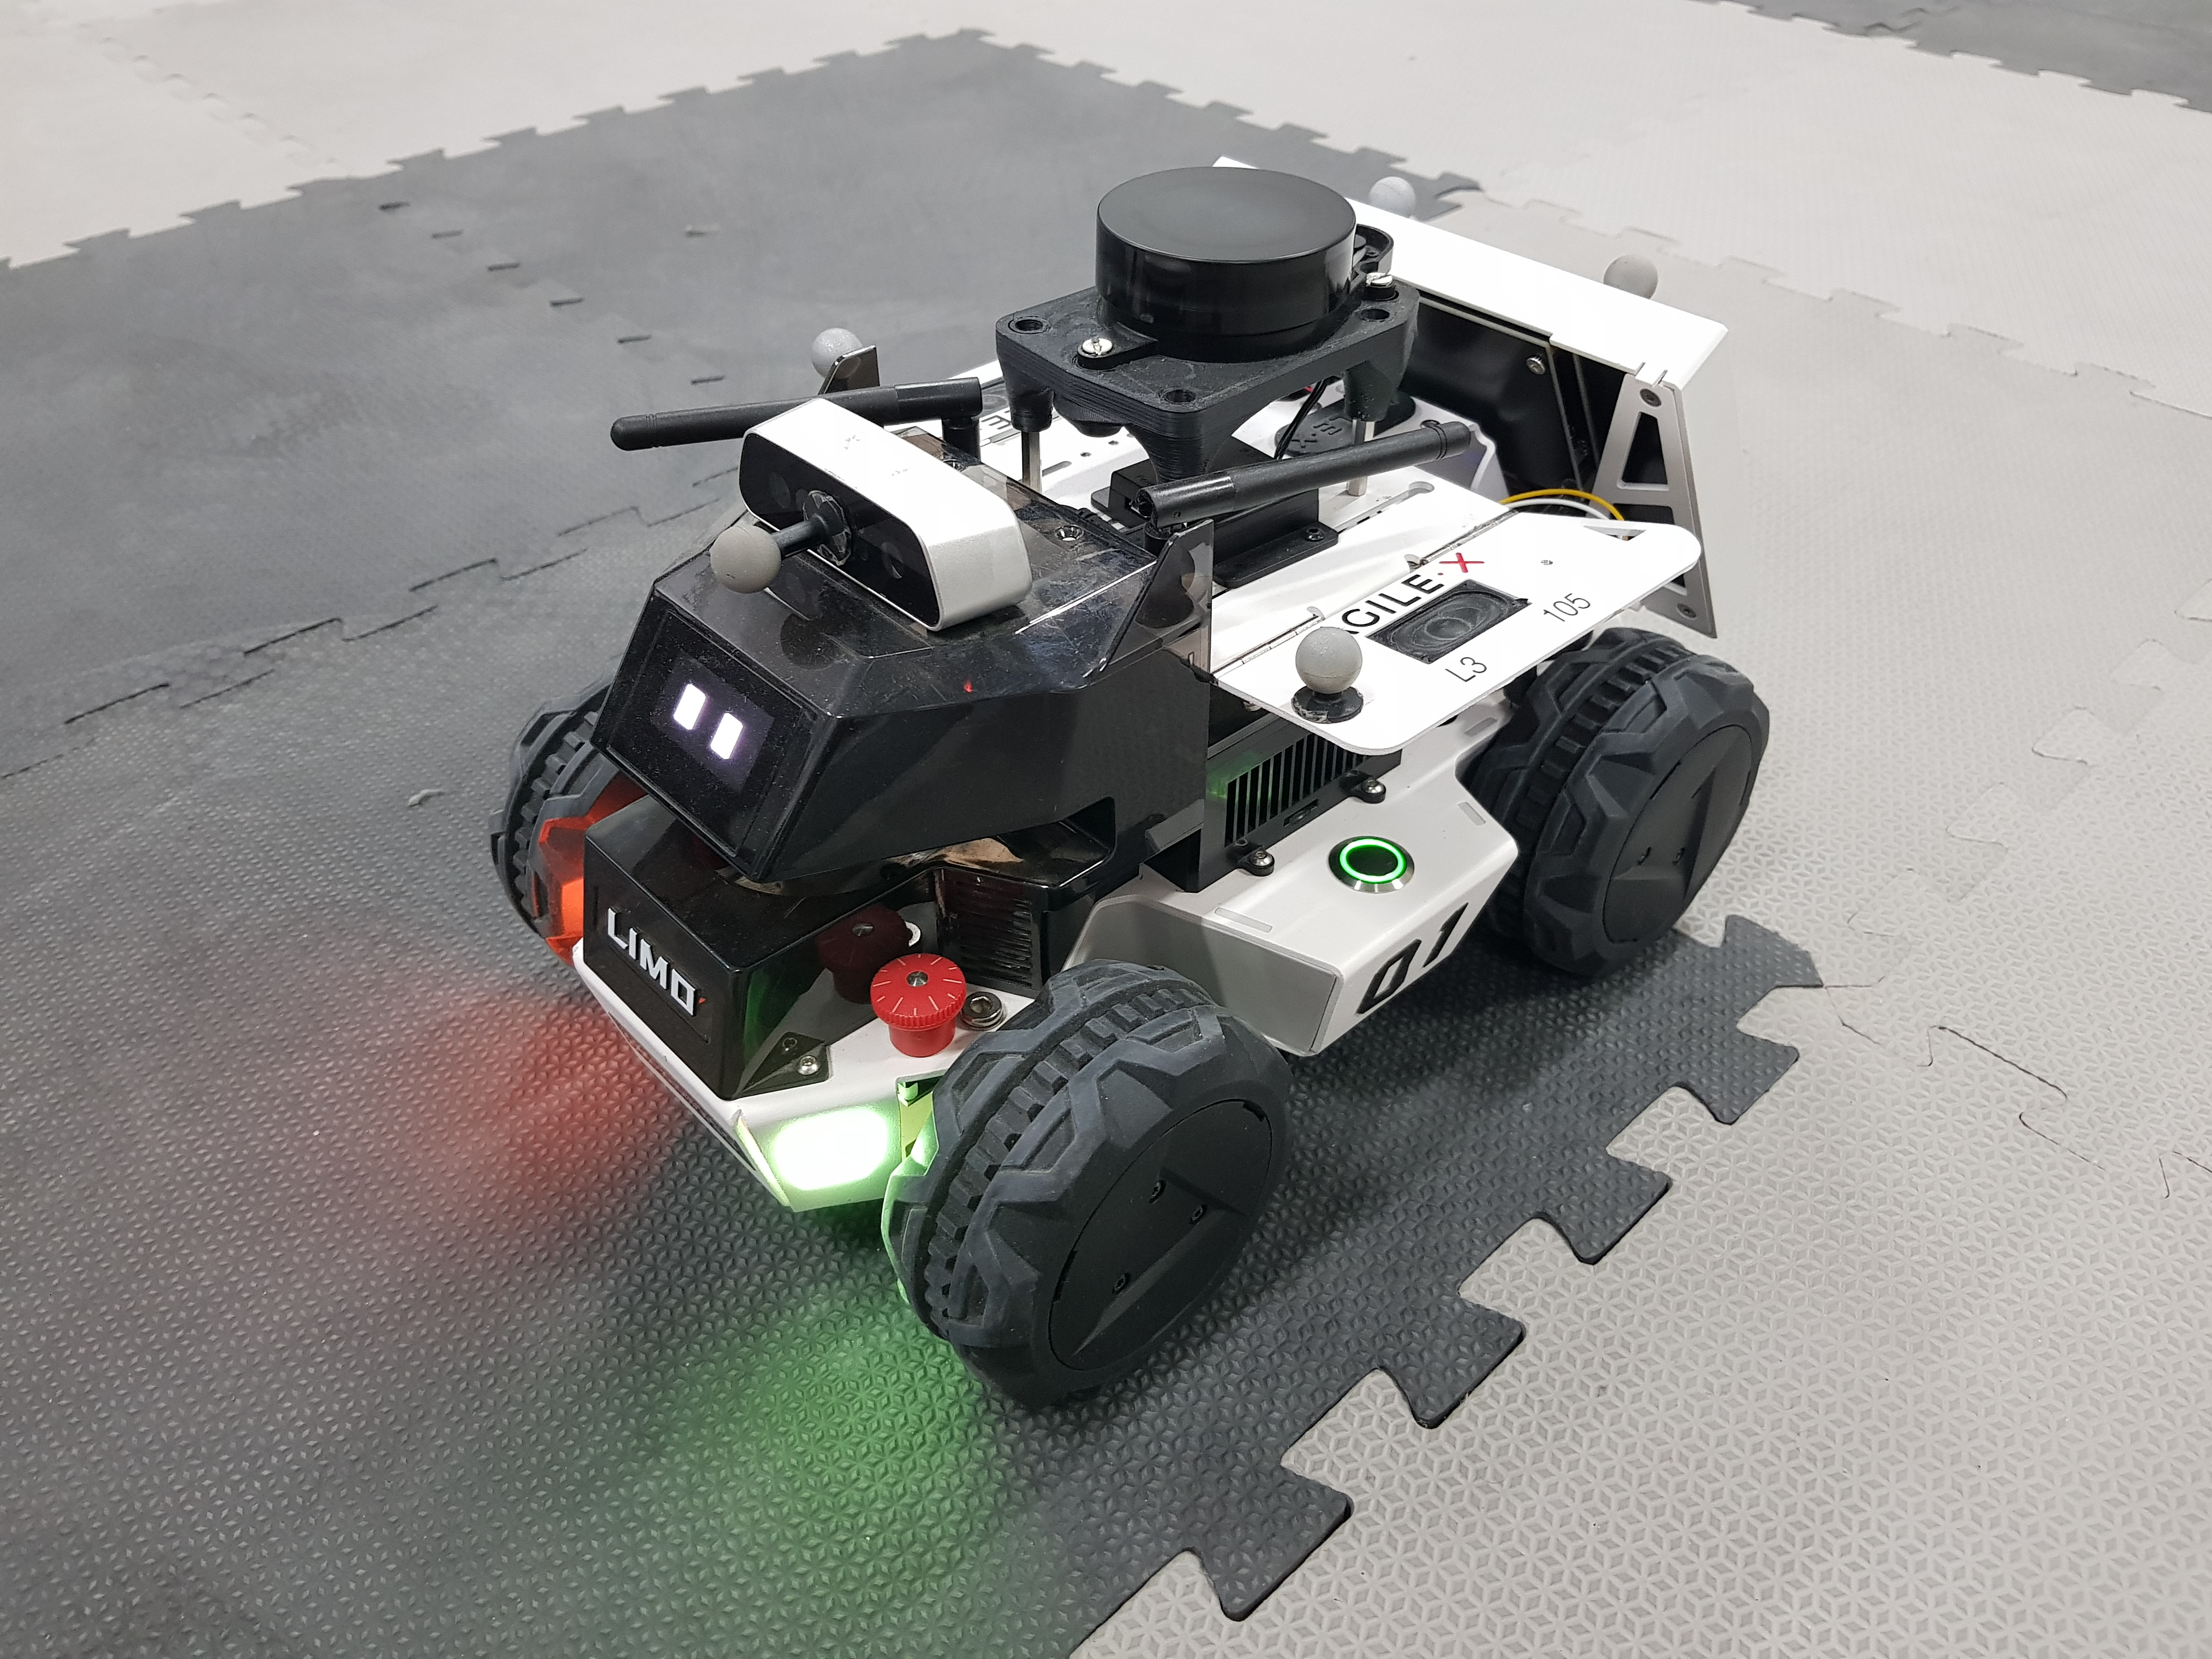
\includegraphics[trim= 700 400 700 150, clip, width=\textwidth]{img/LIMO_EXPERIMENTO.jpg}
        \end{subfigure}
        
        \source
        \label{fig:LIMO_Experimento}
    \end{figure}

    Para realizar o projeto, primeiro foi implementado o controlador para o robô diferencial, seguindo a lei de controle da Equação \ref{eq:ff_fb_law_limo}. O código foi implementado em linguagem C++ e utilizando as bibliotecas do ROS para obtenção dos dados de posição e publicação dos comandos de velocidade.
    
    Também foi implementado um código para publicação da trajetória a ser seguida pelo robô, que calcula os pontos da trajetória em função da frequência de publicação e da velocidade desejada para a trajetória. Este código publica as poses objetivos no tópico \textit{/goal} e também publica o caminho inteiro em um outro tópico, que pode ser utilizado para tarefas de seguimento de caminho ou para visualização da trajetória e/ou caminho desejado. Todos os códigos implementados estão disponíveis no \textit{Github} \cite{site:Github-SLAM_Research}.

    Para a utilização da SLAM Toolbox para este projeto, realizou-se uma cópia do repositório da SLAM Toolbox\cite{site:Slam_toolbox}. Como utilizamos o ROS 1 no LAB-AIR foi necessário modificar o código da SLAM Toolbox para que a pose do robô obtida a partir do escaneamento do LiDAR fosse publicada também no modo de Localização. A SLAM Toolbox somente publicava as poses corretamente na versão para o ROS 2.

    A SLAM Toolbox expõe ao usuário diversos parâmetros de configuração que podem ser modificados para buscar o melhor desempenho do sistema. Para buscar o melhor funcionamento do sistema junto ao controle utilizado e obter melhores resultados, foi necessário modificar estes parâmetros e realizar diversos testes, rodando diversas vezes o código em modo de slam online e localização para obtenção de resultados mais satisfatórios para o projeto. Maiores informações sobre os parâmetros expostos pela biblioteca estão disponíveis no \textit{Github} da biblioteca \cite{site:Slam_toolbox}.
    
    Em específico, notou-se durante a implementação do projeto e durante os testes que o robô utilizado apresentava muitos erros de odometria, devido ao problema de deslizamento das rodas no chão, principalmente ao realizar curvas no modo diferencial. Portanto, para obter melhores resultados utilizando a SLAM Toolbox modificou-se a função utilizada para rejeitar valores discrepantes (\textit{outliers}) para uma função \textit{HuberLoss} através do parâmetro \textit{ceres\_loss\_function}.

    Outros parâmetros também foram alterados para que a pose do robô fosse atualizada e publicada com maior frequência pela biblioteca. Os parâmetros \textit{minimum\_time\_interval}, \textit{minimum\_travel\_distance} e \textit{minimum\_travel\_heading} foram reduzidos para que o sistema de controle pudesse funcionar satisfatoriamente.
    

    

% \section{Estrutura do código}

% \begin{itemize}
%     \item \add{Descrição do sistema original proposto e os algoritmos inicialmente planejados.}
%     \item \add{Justificativa das limitações encontradas e da decisão de adotar o SLAM\_toolbox.}
%     \item \add{Detalhamento da integração do SLAM\_toolbox com os demais módulos do sistema (por exemplo, aquisição e fusão dos dados sensoriais, controle do robô).}
%     \item \add{Descrição da implementação experimental, destacando as etapas de configuração, calibração e execução dos testes.}
% \end{itemize}
